\section{Решение уравнения струны}
\[
	u_{tt} = a^2 u_{xx}
\]
Кроме того, есть граничные условия
\[
	\begin{aligned}
		u(0,t)=0 \\
		u(l,t)=0 
	\end{aligned} ~ \forall t
\]
и начальные
\[
	\begin{aligned}
		u(x,0) = \varphi(x) \\
		u_t(x,0) = \psi(x)
	\end{aligned} ~ x \in [0,l]
\]
Решение Эйлера получается через замену:
\[
	\left\{
	\begin{aligned}
		\xi = at + x \\
		\eta = -at + x
	\end{aligned}
	\right.
\]
решение выражается через $u_{\xi \eta}=0, u=G(\xi) + F(\eta)$.

Решение Даламбера -- ищем стоячие волны $F(x)$, такие, что 
\[
	u(x,t) = \cos \left(\omega t + \chi\right) F(x)
\] являются решением уравнения струны.

Подставим в уравнение:
\[
	\begin{aligned}
	u_{tt}(x,t) = - \omega^2 \cos (\omega t + \chi) F(x)  \\
	u_{xx}(x,t) = \cos (\omega t + \chi) F''(x) \\
	-\omega^2 \cos(\omega t + \chi) F(x) = a^2 \cos(\omega t + \chi) F''(x) \\
	F''(x) + \frac{\omega^2}{a^2} F(x) = 0 \\
	u(0,t) = \cos(\omega t + \chi) F(0) = 0 ~ \forall t \implies F(0) = 0 \\
	F(l) = 0
\end{aligned}
\]
Решаем диффур второго порядка и получаем решение:
\[
	\begin{aligned}
	F(x) = c \sin \frac{\omega}{a} x \\
	F(l) = c \sin \frac{\omega}{a} l = 0 \implies \frac{\omega}{a}l = \pi k, k \in \mathbb{N} \\
	\omega_k = \frac{a \pi}{l} k \\
	F_k (x) = C \sin \left(\frac{\pi k}{l} x\right)
\end{aligned}
\]
Из этого можно получить метод Фурье. Если сложить все $F_k$ в одну функцию, то получится
\[
	u(x,t) = \sum_{k=1}^\infty C_k \cos(\omega_k t+\chi_k)\sin \left( \frac{\pi k}{l} x\right) = \dots
\]
т.е. ряд Фурье. Это будет общее решение.
\[
	\dots = \sum_{k=1}^\infty \left( A_k \cos (\omega_k t) \sin \left( \frac{\pi k}{l} x\right) + B_k \sin (\omega_k t) \sin \left( \frac{\pi k}{l} x\right)\right)
\]
Неизвестными будут $A_k, B_k$. Они подбираются так, чтобы удовлетворить начальным условиям.

Посчитаем полную энергию струны.

\begin{figure}[H]
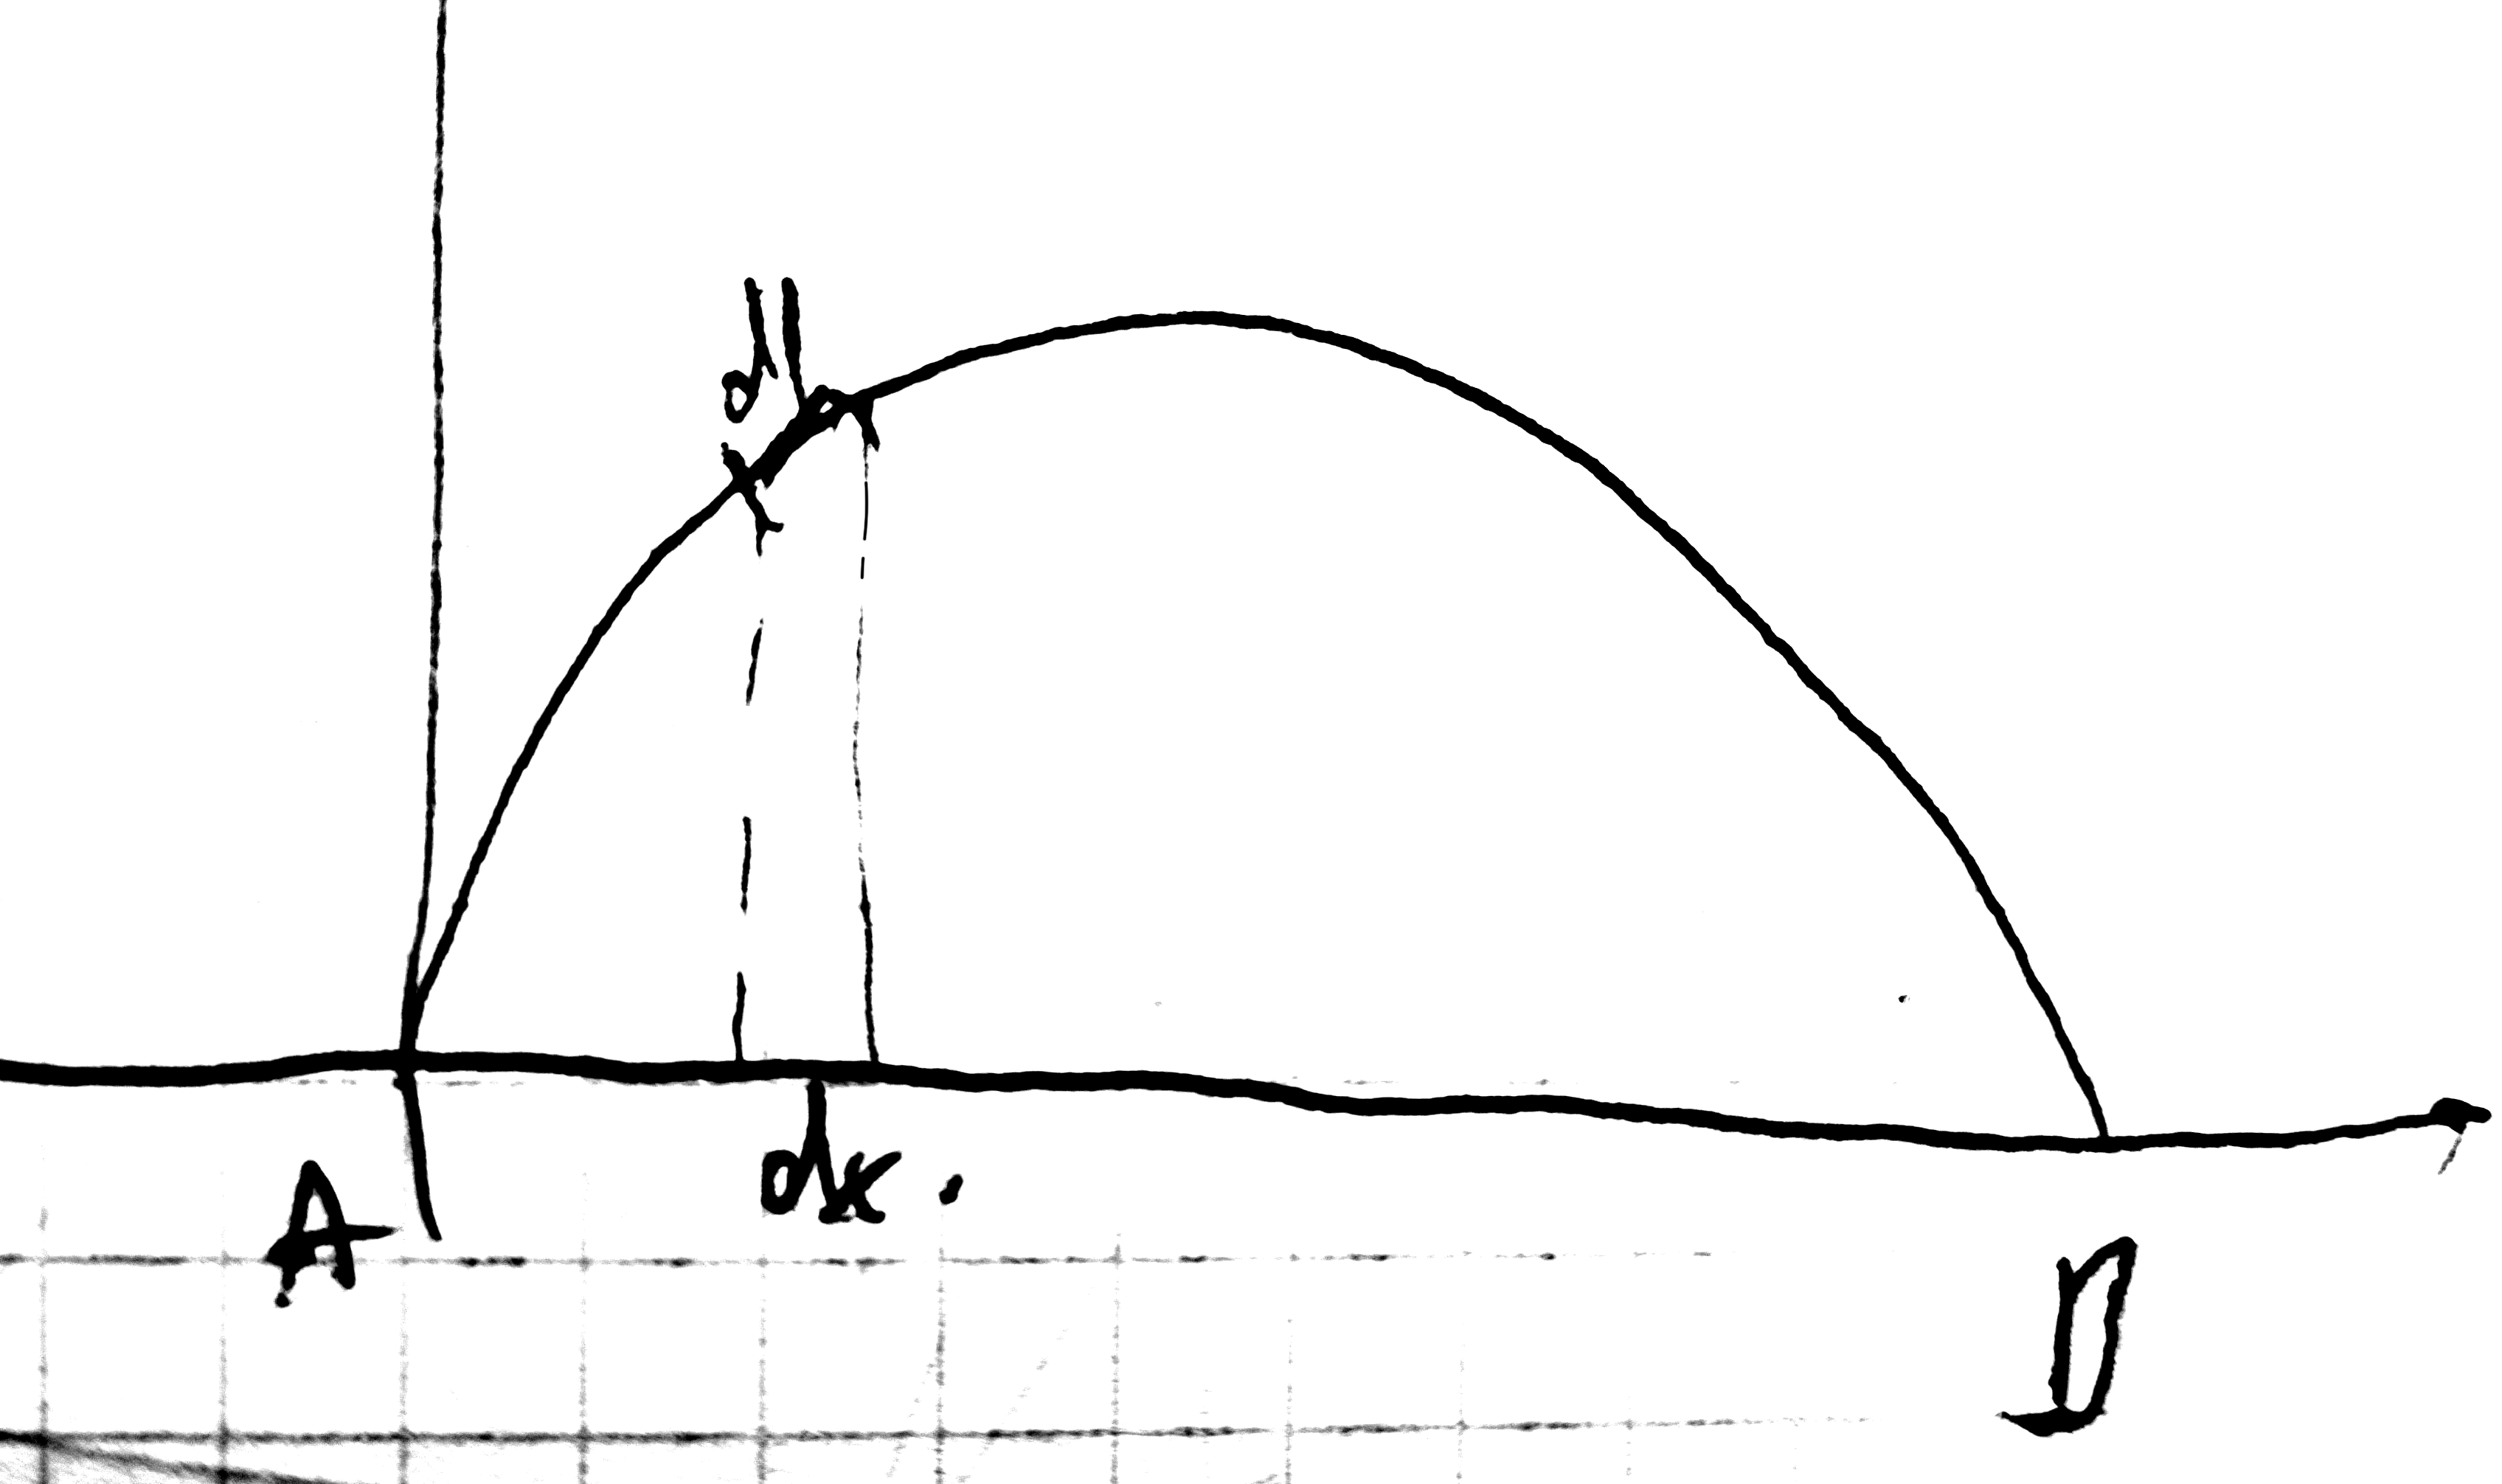
\includegraphics[width=\textwidth]{2}
\end{figure}
\[
	\begin{aligned}
	E = E_\text{К}+E_\text{П} \\
	\mathrm{d}E_\text{К} = \frac{\mathrm{d}m \cdot u_t^2}{2} = \frac{\rho \mathrm{d}l u_t^2}{2} \\
	E_\text{К} = \int\limits_{AB} \frac{\rho \mathrm{d}l \cdot u_t^2}{2} = \int\limits_0^l \frac{\rho u_t^2}{2} \sqrt{1+u_x^2} \mathrm{d}x = \\
	= \frac{\rho}{2} \int\limits_0^l u_t^2 \sqrt{1+u_x^2} \mathrm{d}x \approx \frac{\rho}{2} \int\limits_0^l u_t^2 \mathrm{d}x \\
	\mathrm{d} E_\text{П} = T \underbrace{\left( \mathrm{d}l-\mathrm{d}x\right)}_{\text{удлинение струны}} \\
	E_\text{П} = \int\limits_{AB} T(\mathrm{d}l-\mathrm{d}x) = T \int\limits_0^l \left( \sqrt{1+u_x^2} - 1\right)\mathrm{d}x \approx \\
	\approx \frac{T}{2} \int\limits_0^l u_x^2 \mathrm{d}x \\
	E = E_\text{К} + E_\text{П} \approx \frac{\rho}{2} \int\limits_0^l u_t^2 dx + \frac{T}{2} \int\limits_0^l u_x^2 \mathrm{d}x = \dots\\
	a^2 = \frac{T}{\rho} \implies \\
	\dots = \frac{\rho}{2} \int\limits_0^l \left[ u_t^2 + a^2 u_x^2\right] \mathrm{d}x
\end{aligned}
\]
Рассмотрим тогда функцию вида
\[
	u(x,t) = \cos \left( \omega_k t + \varphi\right) \sin \left( \frac{\omega_k}{a} x\right)
\]
Для неё
\[
	\begin{aligned}
	u_t^2 + a^2 u_x^2 = \omega_k^2 \sin^2 \left( \omega_k t + \varphi\right) \sin^2 \left( \frac{\omega_k}{a} x\right) + \omega_k^2 \cos^2 \left( \omega_k t + \varphi\right)\cos^2 \left( \frac{\omega_k}{a} x\right) = \\
	= \frac{\omega_k^2}{2} + \dots \cos \left( \frac{2 \omega_k}{a} x\right) \\
	E = \frac{\rho}{2} \cdot \frac{\omega_k^2} l = \frac{\rho}{4} \frac{\pi^2 k^2 a^2}{l}
\end{aligned}
\]
Отсюда получается, что чтобы заставить струну колебаться с $k$-й гармоникой, надо $k^2$ энергии.
